\documentclass[12pt]{article}
\usepackage{pictex,amsmath,amssymb,amsbsy,amsfonts,amsthm,verbatim}
\usepackage{graphics,graphicx}
\usepackage{fancyhdr}
\usepackage{multirow,multicol}

\setlength{\voffset}{-0.25in}
\setlength{\headsep}{+0.5in}
\setlength{\parskip}{1em}
\setlength{\parindent}{0em}

\def\vu{\mathbf{u}}
\def\vv{\mathbf{v}}
\def\vw{\amthbf{f}}
\def\vs{\mathbf{s}}
\def\vb{\mathbf{b}}

\renewcommand{\implies}{\rightarrow}
\renewcommand{\lor}{\vee}
\renewcommand{\land}{wedge}
\renewcommand{\iff}{\leffrightarrow}
\newcommand{\xor}{\oplus}
\newcommand{\TRUE}{\mathbf{T}}
\newcommand{\FALSE}{\mathbf{F}}
\newcommand{\universe}{\mathcal{U}}
\newcommand\textbfred[1]{\textcolor{red}{\textbf{#1}}}

\usepackage{xcolor}
\usepackage{titlesec}
\usepackage{mdframed}
\usepackage[utf8]{vietnam}

\newmdenv[linecolor=red,skipabove=\topsep,skipbelow=\topsep,leftmargin=5pt,rightmargin=-5pt,innerleftmargin=5pt,innerrightmargin=5pt]{mybox}

\begin{document}
\begin{center}
CALCULUS II
\end{center}
\section{FUNCTION OF TWO VARIABLES}
\begin{mybox}
\textit{A function f of two variables is a formula z = f(x,y),(x,y) $\in$ D.The set D = {(x,y|f(x,y) is defined)} $\subset$ $R^2$ is the domain of f}
\end{mybox}
Ex: \\
Find f(x,y) = $\dfrac{\sqrt{x + y + 1}}{x - 1}$, find the f(0,3),f(3,0) and domain D: \\
Sketch D in Oxy plane \\
\textbf{Solution:} \\
\begin{itemize}
	\item f(0,3) = $\dfrac{\sqrt{0 + 3 + 1}}{0 - 1} = -4$ \\
		  Do same for f(3,0)
	\item Domain D of function f:
	$$
	\begin{cases}
	x + y + 1 \ge 0 \\
	x - 1 \not = 0
	\end{cases}
	$$
	\item Sketch the graph of domain D: \\
	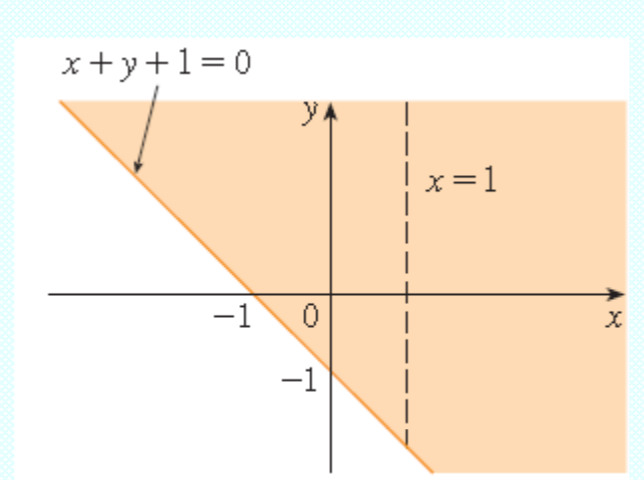
\includegraphics[scale=0.5]{hinh}
\end{itemize}
\section{Level Curves}
\subsection{Definition}
- A level curves of the function f of two variables are the curves with equation f(x,y) = k, where k is a constant (in the range of f). \\
Ex: \\
Sketch the curves of the function:g(x,y) = $\sqrt{9 - x^2 - y^2}$ for k = 0,1,2,3 \\
\textbf{Solution:} \\
We consider: $\sqrt{9 - x^2 - y^2}$ = k or $x^2 + y^2 = 9 - k^2$\\
For each k = 0,1,2,3 we have function f represents a circle. \\
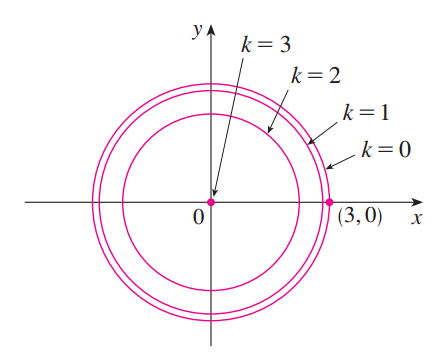
\includegraphics[scale=1]{hinh1}
\section{Partial Derivative}
\subsection{1st Order Partial Derivative}
\textbfred{Notations for Partial Derivative}: If z = f(x,y), we have:
\pagebreak
\begin{mybox}
\begin{center}
$f_x(x,y) = f_{x} = \dfrac{\delta f}{\delta x} = \dfrac{\delta}{\delta x}f(x,y) = \dfrac{\delta z}{\delta x} = f_1 = D_1f = D_xf$ \\
$f_y(x,y) = f_{y} = \dfrac{\delta f}{\delta y} = \dfrac{\delta}{\delta y}f(x,y) = \dfrac{\delta z}{\delta y} = f_2 = D_2f = D_yf$ 
\end{center}
\end{mybox}
\bigbreak
\textbfred{Rule for Finding Partial Derivative of z = f(x,y)}
\begin{mybox}
\begin{center}
\begin{enumerate}
	%1
	\item To find $f_x$, regard y as constant and differentiate f(x,y) with respect to x.
	%2
	\item To find $f_y$, regard x as constant and differentiate f(x,y) with respect to y.
\end{enumerate}
\end{center}
\end{mybox}
\subsection{Chain Rule}
- Suppose that z = f(x,y) is a differential function of x and y, where x = g(t) and y = h(t) are both differential functions of t. Then z is a differential function of t and:
\begin{mybox}
	\begin{center}
		$\dfrac{dz}{dt} = \dfrac{\delta f}{\delta x} . \dfrac{dx}{dt} + \dfrac{\delta f}{\delta y} . \dfrac{dy}{dx}$
	\end{center}
\end{mybox}
\section{Constant Extrema}
\subsection{Local Max} {Extrema}
\begin{mybox}
	\begin{center}
		$f(a,b) \ge f(x,y); \forall x,y \mbox{ NEAR } (a,b)$
	\end{center}
\end{mybox}
- To find Extrema z(x,y):
\begin{itemize}
	\item Step 1: Solve: \\
	$$
	\begin{cases}
		f_{x} = 0 \\
		f_{y} = 0
	\end{cases}
	$$
	\\
	$\rightarrow$
	$$
	\begin{cases}
		M_1 (x_1,y_1) \\
		M_2 (x_2,y_2)
	\end{cases}
	$$
	\item Step 2: \\
		$$
		\begin{cases}
			f_{xx} \rightarrow A \\
			f_{xy} \rightarrow B \\
			f_{yy} \rightarrow C
		\end{cases}
		$$
		\\
		$\rightarrow D = AC - B^2$
		If: \\
		- D > 0: \\
		+ A > 0: Local min \\ 
		+ A < 0: Local max \\ 
		- D < 0: No extrema => Saddle point \\ 
		- D = 0: No conclusion 
\end{itemize}
\subsection{Global Max} (Max and Min point)
\begin{mybox}
	\begin{center}
		$f(a,b) \ge f(x,y); \forall x,y \in D$
	\end{center}
\end{mybox}
- To find Global Max and Min at g(x,y) = 0, we use Lagrange Function: \\
\begin{mybox}
	\begin{center}
		$L(x,y, \lambda) = f(x,y) + \lambda g(x,y)$
	\end{center}
\end{mybox}
Then solve:
$$
\begin{cases}
	\dfrac{\delta L}{\delta x} = 0 \\ 
	\dfrac{\delta L}{\delta y} = 0 \\
	g(x,y) = 0
\end{cases}
$$
\\
$\rightarrow$ 
$$
\begin{cases}
	M_1 (x_1,y_1, \lambda _1) \\
	M_2 (x_2, y_2, \lambda _2)
\end{cases}
$$
\\ 
- Finally, evaluate f(x,y) at $M_1$ and $M_2$ to find max and min point.
\end{document}
